\documentclass[utf8]{beamer}

\usepackage[T1]{fontenc}
\usepackage[brazil]{babel}
\usepackage{inconsolata}
\usepackage{minted}
\usepackage{tabu}
\usepackage[absolute, overlay]{textpos}
\usepackage{graphicx}
\usepackage{changepage} % adjustwidth environment

\definecolor{codebgcolor}{HTML}{FFFFFF}
\definecolor{coderulecolor}{HTML}{5F7FFF}
\definecolor{outerbgcolor}{HTML}{F0F0FF}

\setminted{python3, autogobble,
           breaklines, breakanywhere,
           breaksymbolindentleft=0pt, breaksymbolindentright=0pt,
           breaksymbolsepleft=3pt, breaksymbolsepright=3pt,
           breaksymbolright=...,
           bgcolor=codebgcolor, style=paraiso-light,
           fontsize=\fontsize{8pt}{8pt},
           frame=lines, rulecolor=coderulecolor, framerule=.7pt}
\setmintedinline{bgcolor={}}

\mode<presentation>
\usetheme{Warsaw}
\setbeamercolor{structure}{fg=red!20!black}
\setbeamercolor{background canvas}{bg=outerbgcolor}
\beamertemplatenavigationsymbolsempty

\setbeamertemplate{footline}{\leavevmode\hbox{%
  \begin{beamercolorbox}[wd=.35\paperwidth, ht=2.25ex, dp=1ex, center]
                        {author in head/foot}
    \usebeamerfont{author in head/foot}
      Danilo J. S. Bellini \hfill \texttt{@danilobellini}
  \end{beamercolorbox}%
  \begin{beamercolorbox}[wd=.65\paperwidth, ht=2.25ex, dp=1ex, center]
                        {title in head/foot}
    \usebeamerfont{title in head/foot}
      \insertshorttitle \hfill
      ETEC Uirapuru -- SP \hfill
      \insertshortdate \hfill
      \insertframenumber\,/\,\inserttotalframenumber
  \end{beamercolorbox}%
}}

\title{Segurança da Informação}
\subtitle{Um apanhado geral
          sobre criptografia, acesso e vulnerabilidades,
          incluindo exemplos práticos em Python e Shell}
\author{Danilo J. S. Bellini \\ \texttt{@danilobellini}}
\date{2018-10-18}

\setlength{\TPHorizModule}{\paperheight}
\setlength{\TPVertModule}{\paperheight}

\renewcommand{\thefootnote}{[\arabic{footnote}]}

\newcommand{\includesvg}[2]{%
  \ifnum\pdfstrcmp{\pdffilemoddate{#2.svg}}%
                  {\pdffilemoddate{#2.pdf}}>0%
    {\immediate\write18%
     {inkscape -z -D --file=#2.svg --export-pdf=#2.pdf --export-latex}%
    }%
  \fi%
  \centering%
  \resizebox{#1}{!}{%
    \input{#2.pdf_tex}%
  }%
}


\begin{document}


\begin{frame}
  \titlepage
  \center Semana de informática \\ ETEC Uirapuru -- SP
  \begin{textblock}{0}(.1, .55)%
    
\includegraphics[height=70pt]{logo-etec-uirapuru.png}%
  \end{textblock}
  \begin{textblock}{0}(.8, .55)%
    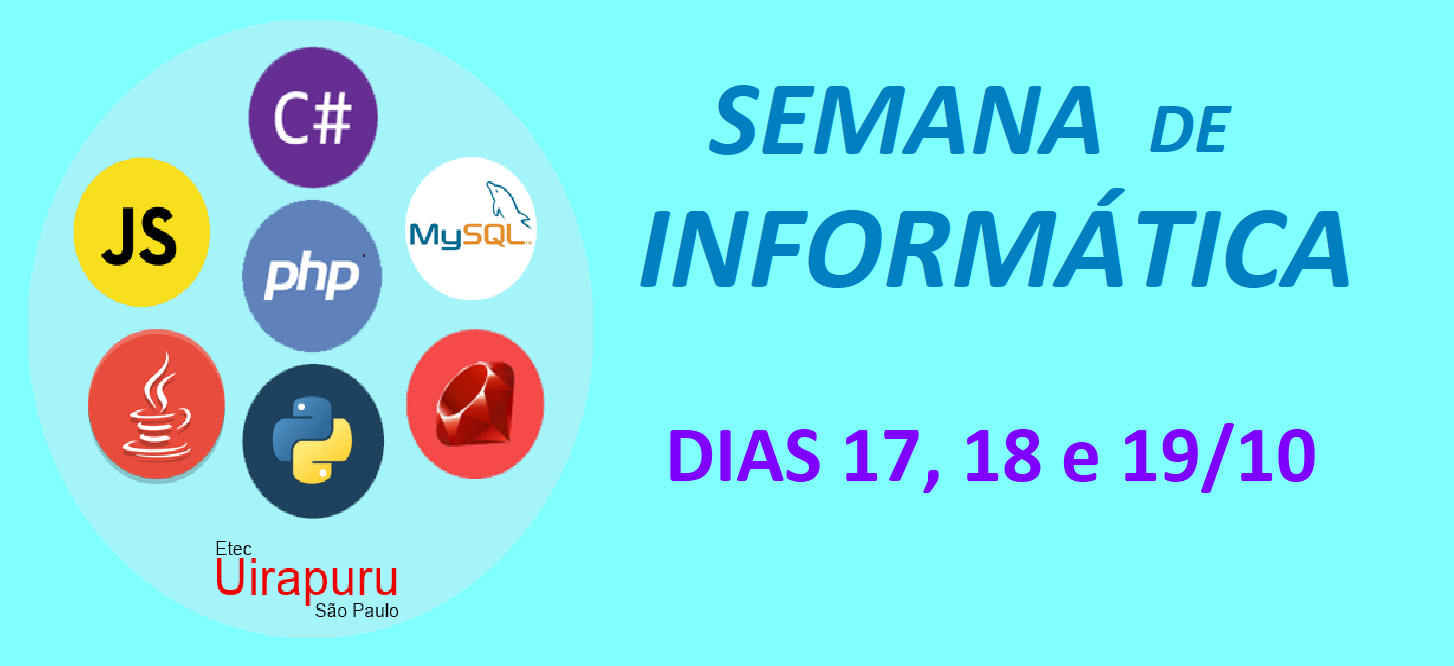
\includegraphics[height=70pt]{banner.png}%
  \end{textblock}
\end{frame}


\begin{frame}{O que é segurança?}
  Estar livre de perigos? Minimizar os riscos?
  \vfill
  Em inglês há duas palavras: safety VS security\footnote{
    Para uma definição mais completa dessas palavras, veja
    \url{http://www.iot.ntnu.no/users/albrecht/rapporter/%
                                notat\%20safety\%20v\%20security.pdf}
  }
  \begin{itemize}
    \item \emph{Safe} refere-se à proteção
          sobre acontecimentos indesejáveis do acaso;
    \item \emph{Secure} refere-se à proteção
          contra acontecimentos intencionais.
          É aqui que se encaixa a segurança da informação.
  \end{itemize}
  \vfill
  Aspectos da segurança da informação:
  \begin{itemize}
    \item Confidencialidade / Privacidade
    \item Integridade
    \item Disponibilidade
  \end{itemize}
  \begin{textblock}{0}(.85, .6)%
    \includesvg{110pt}{Crypto_key}%
  \end{textblock}
\end{frame}


\begin{frame}{Criptografia}
  Criptografia é a prática e o estudo
  das técnicas de armazenamento e comunicação de informação
  na presença de terceiros/adversários.
  \vfill
  Técnicas tradicionais incluem:
  \begin{itemize}
    \item Criptografia de chave simétrica
          (chave única, de conhecimento exclusivo das partes)
    \item Criptografia de chave pública
          (pares de chave pública/privada para cada parte)
    \item Funções de \emph{hash} (sem chave)
  \end{itemize}
  \vfill
  Objetivos:
  \begin{itemize}
    \item \emph{Sign}, assinatura (integridade)
    \item \emph{Encrypt/Decrypt}, encriptação/decriptação
          (confidencialidade)
  \end{itemize}
\end{frame}


\begin{frame}[fragile]{Cifras de César, Vigenère e autochave}
  \begin{columns}[c]
    \column{.6\textwidth}
    Cifra de César (possui 1 parâmetro)
    \resizebox{\textwidth}{!}{%
      \begin{tabular}{rl}
             Mensagem: & \texttt{EU GOSTO DE LIMONADA} \\ \hline
                Chave: & \texttt{C} (desloca 2 no alfabeto) \\
        Texto cifrado: & \texttt{GW IQUVQ FG NKOQPCFC}
      \end{tabular}%
    }
    \vspace{.5em}\vfill
    Cifra de Vigenère (chave simétrica)
    \resizebox{\textwidth}{!}{%
      \begin{tabular}{rl}
             Mensagem: & \texttt{EU GOSTO DE LIMONADA} \\ \hline
                Chave: & \texttt{MENTIRA} \\
        Chave efetiva: & \texttt{ME NTIRA ME NTIRAMEN} \\
        Texto cifrado: & \texttt{QY THAKO PI YBUFNMHN} \\ \hline
                Chave: & \texttt{PAGAZAQ} \\
        Chave efetiva: & \texttt{PA GAZAQ PA GAZAQPAG} \\
        Texto cifrado: & \texttt{TU MORTE SE RILODPDG}
      \end{tabular}
    }
    \vspace{.5em}\vfill
    Autochave (chave simétrica)
    \resizebox{\textwidth}{!}{%
      \begin{tabular}{rl}
             Mensagem: & \texttt{EU GOSTO DE LIMONADA} \\ \hline
                Chave: & \texttt{PAGAZAQP} \\
        Chave efetiva: & \texttt{PA GAZAQ PE UGOSTODE} \\
        Texto cifrado: & \texttt{TU MORTE SI FOAGGOGE}
      \end{tabular}%
    }

    \column{.5\textwidth}
    A cifra de César transforma cada caractere da mensagem
    usando esta tabela:
    \vspace{.5em}\vfill
    \resizebox{\textwidth}{!}{%
      \begin{tabular}{c|c|c|c|c|c}
        \texttt{A} \textrightarrow \texttt{C} &
        \texttt{B} \textrightarrow \texttt{D} &
        \texttt{C} \textrightarrow \texttt{E} &
        \texttt{D} \textrightarrow \texttt{F} &
        \texttt{E} \textrightarrow \texttt{G} &
        \texttt{F} \textrightarrow \texttt{H} \\
        \texttt{G} \textrightarrow \texttt{I} &
        \texttt{H} \textrightarrow \texttt{J} &
        \texttt{I} \textrightarrow \texttt{K} &
        \texttt{J} \textrightarrow \texttt{L} &
        \texttt{K} \textrightarrow \texttt{M} &
        \texttt{L} \textrightarrow \texttt{N} \\
        \texttt{M} \textrightarrow \texttt{O} &
        \texttt{N} \textrightarrow \texttt{P} &
        \texttt{O} \textrightarrow \texttt{Q} &
        \texttt{P} \textrightarrow \texttt{R} &
        \texttt{Q} \textrightarrow \texttt{S} &
        \texttt{R} \textrightarrow \texttt{T} \\
        \texttt{S} \textrightarrow \texttt{U} &
        \texttt{T} \textrightarrow \texttt{V} &
        \texttt{U} \textrightarrow \texttt{W} &
        \texttt{V} \textrightarrow \texttt{X} &
        \texttt{W} \textrightarrow \texttt{Y} &
        \texttt{X} \textrightarrow \texttt{Z} \\
        \texttt{Y} \textrightarrow \texttt{A} &
        \texttt{Z} \textrightarrow \texttt{B}
      \end{tabular}%
    }
    \vfill
    \begin{minted}{python}
      # Código das funções no próximo slide
      msg = "EU GOSTO DE LIMONADA"
      cesar(msg, key="C")
      vigenere(msg, key="MENTIRA")
      vigenere(msg, key="PAGAZAQ")
      autokey(msg, key="PAGAZAQP")
    \end{minted}
    \vfill
    \emph{Desafio}: escrever uma função para cada algoritmo de cifra
                    que encontra o texto original
                    dados a chave e o texto cifrado.
  \end{columns}
\end{frame}


\begin{frame}[fragile]{Cifra de César, Vigenère e autochave em Python}
  \begin{minted}{python}
    from itertools import cycle, accumulate
    from string import ascii_uppercase as alphabet

    def shift_table(key):
        idx = alphabet.find(key)
        return str.maketrans(alphabet, alphabet[idx:] + alphabet[:idx])

    def cesar(msg, key):
        return msg.translate(shift_table(key))

    def vigenere(msg, key):
        parts = msg.split() ; joined = "".join(parts)
        chars = [ch.translate(shift_table(k))
                 for ch, k in zip(joined, cycle(key))]
        positions = accumulate(map(len, parts[:-1]))
        for end in list(positions)[::-1]:
            chars.insert(end, " ")
        return "".join(chars)

    def autokey(msg, key):
        parts = msg.split() ; joined = "".join(parts)
        chars = [ch.translate(shift_table(k))
                 for ch, k in zip(joined, key + joined)]
        positions = accumulate(map(len, parts[:-1]))
        for end in list(positions)[::-1]:
            chars.insert(end, " ")
        return "".join(chars)
  \end{minted}
\end{frame}


\begin{frame}{Chave pública/privada}
  Analogia:
  \begin{adjustwidth}{2em}{1em}\emph{
    Envio pelo correio um cadeado aberto sem a chave,
    o destinatário recebe,
    tranca um pacote com o cadeado e envia p/ mim.
  }\end{adjustwidth}
  Nesse exemplo, o cadeado desempenha o papel de chave pública,
  e a chave do cadeado desempenha o papel de chave privada.
  \vfill
  Vamos ver:
  \begin{itemize}
    \item
    um algoritmo de chave pública/privada
    utilizado para troca de chave simétrica
    \item
    um exemplo prático de uso de chave pública/privada
    no OpenPGP\footnote{
      PGP significa \emph{Pretty Good Privacy},
      um software comercial criado em 1991.
      Sua segunda versão tornou-se o [hoje obsoleto] padrão RFC1991.
      A menos de uma atualização relativa ao algoritmo Camellia,
      RFC4880 (OpenPGP) é a versão mais recente do padrão.
    }.
  \end{itemize}
\end{frame}


\begin{frame}[fragile]{Diffie-Hellman:
                       Exemplo de algoritmo para troca de chave}
  \begin{columns}[c]
    \column{.5\textwidth}
    \includesvg{\textwidth}{Diffie-Hellman_Key_Exchange}

    \column{.5\textwidth}
    \resizebox{\textwidth}{!}{%
      \begin{tabular}{rl}
        Número primo (público): & $p$ \\
        Base (público): & $g$ \\
        Chave privada da Alice: & $a$ \\
        Chave pública da Alice: & $A = g^a \mod p$ \\
        Chave privada do Bob: & $b$ \\
        Chave pública do Bob: & $B = g^b \mod p$ \\
        Número compartilhado: & $A^b \equiv B^a \mod p$
      \end{tabular}%
    }
    \vspace{.5em}\vfill
    Exemplo:
    \begin{minted}{python}
      # Alice e Bob combinam os parâmetros
      p = 2551
      g = 2

      # Criam chaves privadas em silêncio
      a = 45
      b = 29

      # Calculam e trocam chaves públicas
      A = (g ** a) % p          # 2285
      B = (g ** b) % p          # 207

      # Alice e Bob possuem um segredo!
      secret = (A ** b) % p     # 414
      secret = (B ** a) % p     # 414
    \end{minted}
  \end{columns}
\end{frame}


\begin{frame}[fragile]{GPG~-- \emph{GNU Privacy Guard}}
  O GPG é uma implementação em software livre (GPLv3)
  que atende ao OpenPGP
  sem utilizar softwares/algoritmos patenteados/restritos/privados.
  \begin{minted}{shell}
    gpg --gen-key # Criar chaves (par público/privado)
    gpg -k        # Visualizar chaves disponíveis

    # Exportando/importanto chaves públicas (para um dado keyID)
    gpg --keyserver pgp.mit.edu --send-keys keyID
    gpg --keyserver pgp.mit.edu --recv-keys keyID
    gpg --export --armor danilo.bellini@gmail.com > my.key
    gpg --import my.key

    # Assinatura
    gpg -b message.txt                       # Assina (cria ".sig")
    gpg --verify message.txt.sig message.txt # Verifica assinatura

    # Codificando/criptografando (crypt) p/ um destinatário específico
    gpg -o encrypted.gpg -r danilo.bellini@gmail.com -e message.txt

    # Decodificando/decriptografando (decrypt) com a chave privada
    gpg -o decrypted.txt -d encrypted.gpg

    # Comandos utilizados na apresentação (além de vim, cat, rm, ...)
    seq 15 > message.txt     # Cria message.txt c/ sequência de 1 a 15
    hexdump -C encrypted.gpg # Visualizando arquivos como binários
  \end{minted}
\end{frame}


\begin{frame}[fragile]{Tomb: armazenamento criptografado em um arquivo}
  Discos rígidos, SSDs, SDs e outras mídias
  normalmente não estão criptografados.
  \emph{Tomb} permite criarmos diretórios criptografados
  com uma chave criptografada com GPG escondida em uma imagem.
  \vfill
  \begin{minted}{shell}
    tomb dig new.tomb -s 50          # Cria o new.tomb com 50MB
    tomb forge new.key -g            # Cria uma chave encriptada com GPG
    tomb lock new.tomb -k new.key -g # Atribui a chave e formata o new.tomb

    tomb open new.tomb -k new.key -g # Monta o new como se fosse um pendrive
    tomb close new                   # Desmonta o new

    # Esteganografia
    cp EnigmaMachine.jpg new.jpg     # Cópia para não perder a imagem original
    tomb bury new.jpg -k new.key -g  # Armazena chave (+ senha) na imagem
    tomb exhume new.jpg -k copy.key  # Extrai a chave da imagem
    tomb open new.tomb -k new.jpg -g # Podemos usar a imagem direto
  \end{minted}
  \vfill
  \begin{columns}[c]
    \column{.15\textwidth}
    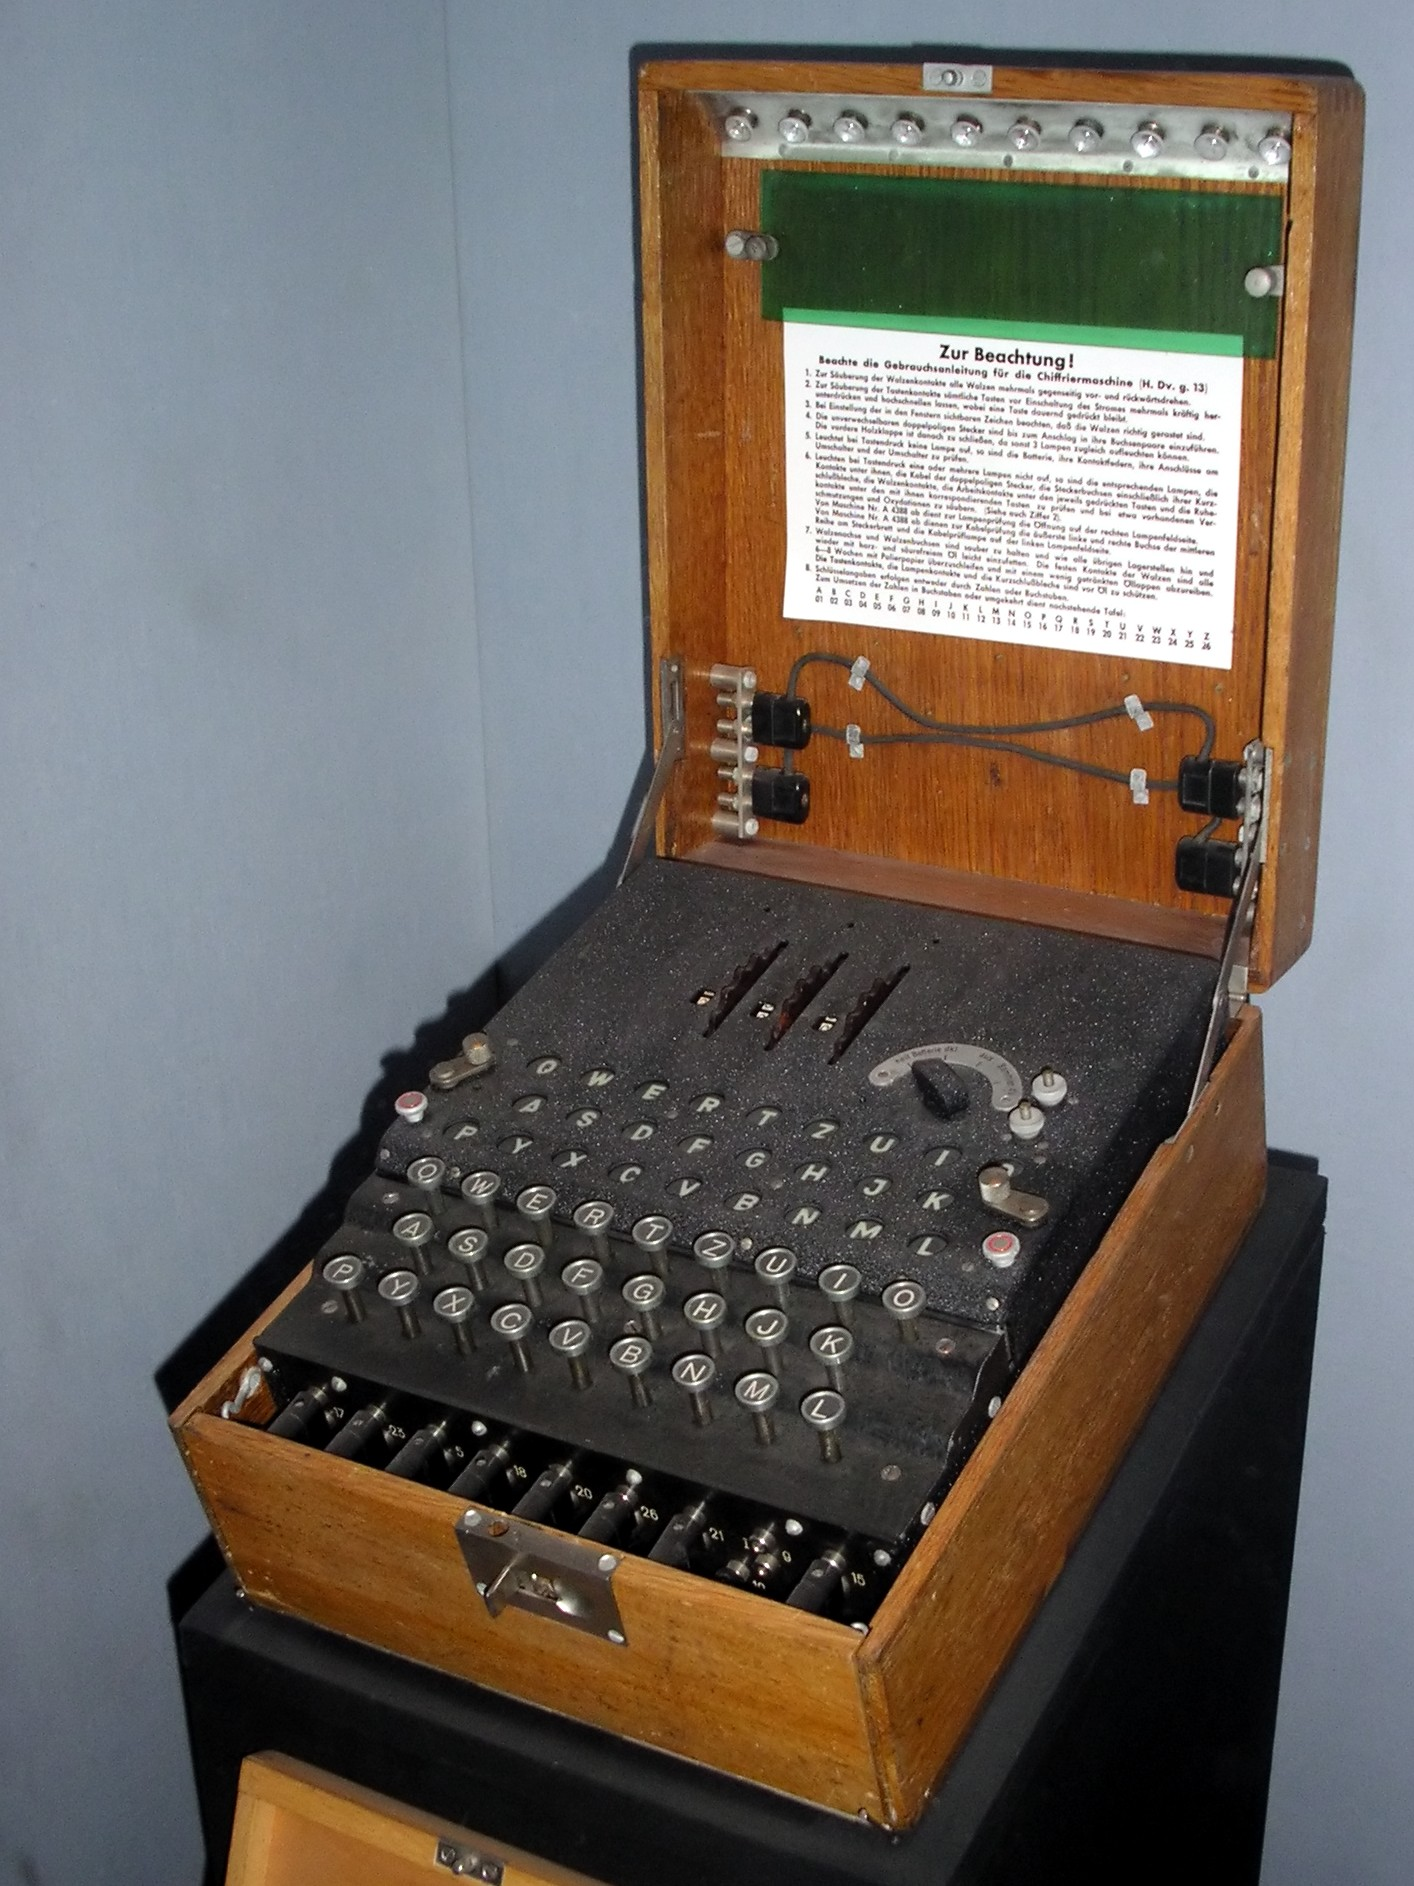
\includegraphics[height=60pt]{EnigmaMachine.jpg}
    \column{.85\textwidth}
    \centering
    Quem imaginaria que a imagem ao lado poderia conter uma chave?
    \vfill
    Use senhas fortes (mais sobre isso em breve)!
  \end{columns}
\end{frame}


\begin{frame}{\emph{Hash},
              funções de espalhamento ou dispersão criptográfica}
  Um valor ou código \emph{hash}
  (também conhecido como \emph{digest} ou ``resumo'')
  é o resultado de uma função de \emph{hash} para uma dada mensagem.
  No contexto da criptografia, funções de \emph{hash} são:
  \begin{itemize}
    \item Determinísticas
          (mesma mensagem $\Rightarrow$ mesmo \emph{hash})
    \item ``Caóticas'' (pequenas mudanças na entrada
                        mudam o hash completamente)
    \item Extremamente difíceis de reverter
          (somente podemos obter a mensagem a partir do hash
           por tentativa e erro)
    \item Extremamente difíceis de colidir
          (idealmente nunca encontramos
           mensagens diferentes com o mesmo \emph{hash})
  \end{itemize}
  \vfill
  Exemplos de algoritmos:
  \begin{itemize}
    \item Checksum e dígitos verificadores (CPF, RG, ISSN, etc.)
    \item MD5 (foi quebrado, útil para fins didáticos)
    \item SHA-1 (usado em torrents, git, etc.;
                 teve uma custosa colisão intencional de hashes de PDFs
                 no \emph{SHAttered})
    \item SHA-2 (há $6$ funções diferentes:
                 SHA-224, SHA-256, SHA-384, SHA-512,
                 SHA-512/224, SHA-512/256)
  \end{itemize}
\end{frame}


\begin{frame}[fragile]{Hashes no Linux}
  \begin{minted}{shell}
    $ echo "O segredo é *#(U*#E, não conta para ninguém" > msg.txt

    $ md5sum msg.txt
    30a4e40dc44b8d1579a086f3e54cb165  msg.txt

    $ sha1sum msg.txt
    df9da1b3ec550a0ae39e70c3d455940fbd74efa1  msg.txt

    $ sha224sum msg.txt
    99ef0cc5ba6a58bbee572cc2527dc469d8c9ea0998885ebe0e558c0b  msg.txt

    $ sha256sum msg.txt
    0b9b5d4b7dcee9fa58653e4e782abf8f40da985d77467f47c9e44848ad43b4d3  msg.txt

    # Todos possuem validação com -c

    $ md5sum -c <<< "30a4e40dc44b8d1579a086f3e54cb165 msg.txt"
    msg.txt: OK

    $ md5sum -c <<< "30a4e40dc44b8d1579a086f3e54cb167 msg.txt"
    msg.txt: FAILED
    md5sum: WARNING: 1 computed checksum did NOT match
  \end{minted}
\end{frame}


\begin{frame}[fragile]{Hashes em Python}
  \begin{minted}{python}
    >>> import hashlib                  # Biblioteca padrão
    >>> with open("msg.txt", "rb") as msg_file:
    ...     msg = msg_file.read()
    ...
    >>> hashlib.md5(msg).hexdigest()    # Hashes como strings comuns
    '30a4e40dc44b8d1579a086f3e54cb165'
    >>> hashlib.sha256(msg).hexdigest()
    '0b9b5d4b7dcee9fa58653e4e782abf8f40da985d77467f47c9e44848ad43b4d3'
    >>> hashlib.sha224(msg).hexdigest()
    '99ef0cc5ba6a58bbee572cc2527dc469d8c9ea0998885ebe0e558c0b'
    >>> hashlib.sha1(msg).hexdigest()
    'df9da1b3ec550a0ae39e70c3d455940fbd74efa1'
  \end{minted}
  \vfill
  \begin{columns}[c]
    \column{.8\textwidth}
    \centering
    Tá legal, verificar \emph{hashes} valida
    a integridade da mensagem,
    seja ela um texto, um arquivo ou um pedaço de um arquivo...
    mas como é que isso pode ajudar na confidencialidade?
    \column{.2\textwidth}
    \includesvg{\textwidth}{Sha-family}
  \end{columns}
\end{frame}


\begin{frame}{Certificados da Python Sudeste}
  Objetivo:
  \begin{itemize}
    \item Gerar certificados personalizados por tipo de participação
          (possivelmente mais de um certificado por pessoa)
    \item Autenticar certificados por parte de quem possui o código
          e outras informações fundamentais
    \item Código $100\%$ \emph{open source}
    \item Utilizar somente dados públicos, apenas em um front-end
          (não há banco de dados,
           o servidor é o de páginas estáticas no GitHub)
    \item Não tornar pública a lista de participantes (privacidade)
  \end{itemize}
  \vfill
  A solução adotada utilizou SHA-3.
  A lista de hashes que autenticam um certificado é pública,
  porém os códigos estão associados
  a outras informações necessárias para autenticar,
  e é extremamente custoso verificar as combinações por força bruta.
\end{frame}


\begin{frame}{Senhas}
  Existem duas tarefas para as quais
  credenciais de acesso são necessárias:
  \begin{itemize}
    \item Autenticação: identificação de quem está solicitando
    \item Autorização: verificação o solicitante tem permissão
                       de realizar determinada solicitação
  \end{itemize}
  \vfill
  Senhas ``fortes'' são importantes para, no mínimo,
  evitarmos o ataque por \emph{brute force} (força bruta),
  que consiste em tentar adivinhar a senha por tentativa e erro,
  exaustivamente.
  Muitos sistemas bloqueiam repetidas tentativas de acesso
  e/ou dificultam o processo com CAPTCHAs,
  mas o ideal é não precisar depender disso.
  \vfill
  Uma forma de ataque, chamada de \emph{ataque de dicionário},
  consiste em algo similar à força bruta,
  mas restrito àquilo que são consideradas escolhas mais prováveis:
  data de nascimento, data de casamento,
  algum evento considerado importante, nome de parente,
  nomes de animais, ideias, projetos, filmes/livros favoritos, etc..
\end{frame}


\begin{frame}
  \centering
  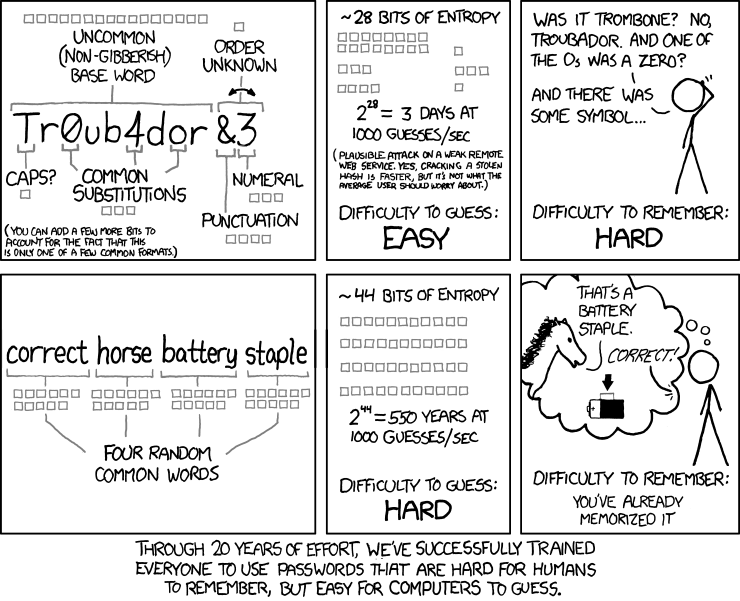
\includegraphics[width=.8\textwidth]{password_strength.png}
  \url{https://www.xkcd.com/936/}
  \vfill
  São $\approx 44$ bits se considerarmos mensagens de $4$ palavras
   em um universo de $2000$ palavras equiprováveis
\end{frame}


\begin{frame}{Políticas para escolha de senhas}
  \begin{columns}[c]
    \column{.5\textwidth}
    \begin{itemize}
      \item Não saia chutando todas as senhas que você usa,
            alguém pode estar gravando tudo
      \item Não deixe senhas trafegar a rede sem criptografia
            (verifique o ``cadeado verde'' no navegador)
      \item Nunca utilize a mesma senha em dois sistemas diferentes,
            do contrário correrá o risco de que alguém de um sistema
            consiga acessar sua conta do outro sistema
    \end{itemize}
    \column{.5\textwidth}
    Memorizar muitas senhas fortes não é fácil.
    Quando precisamos trocá-las com frequência
    (o que não é recomendado),
    a tendência é que as enfraquecemos cada vez mais,
    ou adotamos procedimentos inapropriados:
    \begin{itemize}
      \item Enviar e-mail/mensagem com a senha para si próprio
      \item Colar um \emph{post-it} na tela do computador com a senha
    \end{itemize}
  \end{columns}
\end{frame}


\begin{frame}
  \begin{columns}[c]
    \column{.5\textwidth}
    \centering
    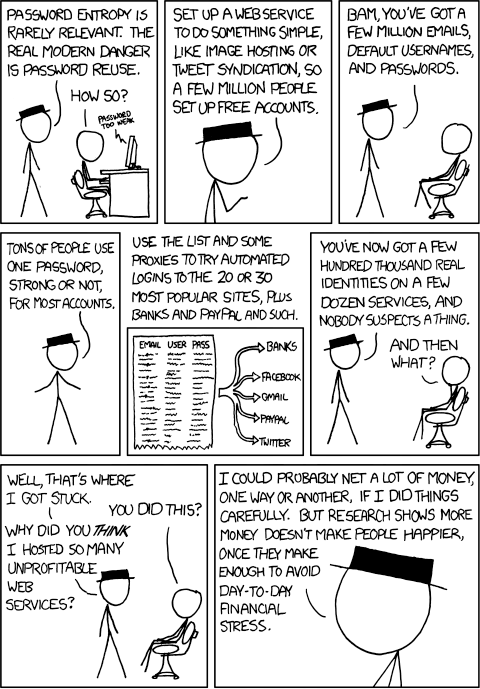
\includegraphics[width=\textwidth]{password_reuse_1.png}
    \column{.5\textwidth}
    \centering
    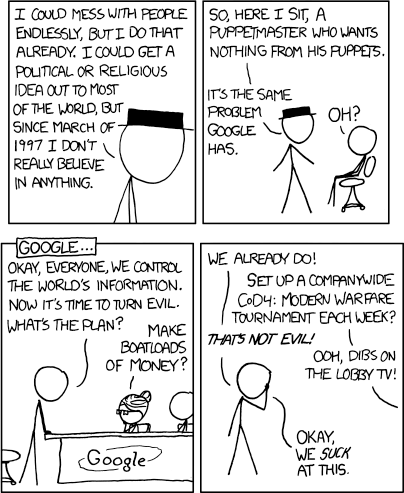
\includegraphics[width=\textwidth]{password_reuse_2.png}
    \url{https://www.xkcd.com/792/}
  \end{columns}
\end{frame}


\begin{frame}{Armazenamento de senhas e \emph{password managers}}
  O que queremos com a senha?
  \begin{itemize}
    \item Validar para fins de autenticação ou autorização?
          Não precisamos da senha,
          precisamos apenas de um validador (\emph{hash}).
    \item Fornecer para outro sistema? Preciso da senha!
  \end{itemize}
  \vfill
  Como poderíamos armazenar um validador de senhas?
  Apenas para validar, o ideal seria não guardar a senha.
  \vfill
  Podemos usar funções de hash!
  A senha pode ser justaposta
  com um bloco constante (denominado \emph{salt} ou \emph{nonce}),
  e armazenamos apenas o hash do resultado.
  Se a mesma senha for fornecida duas vezes,
  o resultado precisa ser igual, o que basta para validar.
  \vfill
  Porém, softwares \emph{password managers} não têm alternativa,
  a não ser armazenarem a senha.
  Como nossas senhas são armazenadas, quem acessa,
  e como elas trafegam a rede?
  São realmente softwares em que podemos confiar?
\end{frame}


\begin{frame}
  \centering
  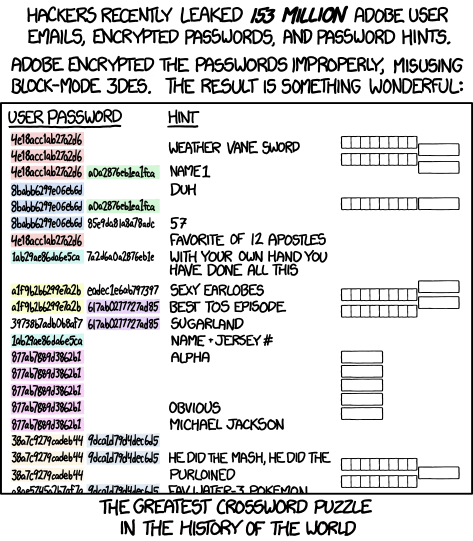
\includegraphics[width=.7\textwidth]{encryptic.png}
  \url{https://www.xkcd.com/1286/}
\end{frame}


\begin{frame}{OTP: \emph{one time password}}
  OTP são senhas de uso único,
  as quais posteriormente são descartáveis.
  Códigos enviados por SMS ou gerados por um aplicativo
  para liberar um acesso são exemplos de tais senhas.
  \vfill
  Podem ser gerados de diferentes formas,
  mas costumam ser hashes sobre um token fixo e alguma
  informação adicional como:
  \begin{itemize}
    \item Instante atual (e.g. TOTP\footnote{
      RFC6238, \emph{Time-based OTP}, uma extensão do HOTP
    })
    \item Contador (e.g. HOTP\footnote{
      RFC4226, \emph{HMAC-based OTP}
    })
    \item OTP anterior (chain)
    \item Aleatório (necessita armazenamento no servidor)
  \end{itemize}
  \vfill
  O mais comum é o TOTP de 6 dígitos\footnote{
    Dígitos menos significativos,
    recomendação do apêndice E do RFC4226.
  }.
\end{frame}


\begin{frame}[fragile]{Pass: \emph{The Standard Unix Password Manager}}
  \begin{columns}[c]
    \column{.8\textwidth}
    Pass é um software livre (GPLv2+), um gerenciador de senhas
    com armazenamento das senhas em um repositório \emph{git} local
    criptografado com GPG.
    \column{.2\textwidth}
    \centering
    
\includegraphics[width=.8\textwidth]{fake.png}
    \vfill
    \fontsize{7pt}{7pt}\selectfont
    QRcode ``fraco'' p/ TOTP
  \end{columns}
  \vfill
  \begin{minted}{shell}
    pass init # Cria o repositório git em ~/.password-store
    pass      # Listar árvore de nomes de arquivos no repositório (não senhas)

    pass generate twitter        # Gerar senha no arquivo "twitter"
    pass generate -n facebook 18 # 18 caracteres, sem caracteres especiais
    pass generate -c email       # "-c" copia para a área de transferência

    pass edit facebook # Edição da senha em editor
    pass insert etec   # Inserção manual (também pode sobrescrever)

    pass mv etec etec.uirapuru # Renomear (mover arquivo)
    pass rm facebook           # Remover

    pass email      # Acesso à senha
    pass -c twitter # "-c" copia para a área de transferência

    # TOTP (com qrencode, zbar e plugin pass-otp)
    qrencode -o fake.png 'otpauth://totp/noone@nowhere?secret=AAAA&issuer=fake'
    zbarimg -q --raw fake.png | pass otp insert fake
    pass otp fake # Geração do TOTP (c/ -c copia na área de transferência)
  \end{minted}
\end{frame}


\begin{frame}{2FA e MFA: \emph{multi-factor authentication}}
  MFA significa usar mais de um fator
  durante um processo de autenticação.
  2FA é o MFA com exatos $2$ fatores.
  \vfill
  ``Verbos'' categorizando possíveis fatores:
  \begin{itemize}
    \item ``Conhecer'':
          Senhas, PIN (\emph{personal identification number}),
          questões sobre a vida/moradia da pessoa
    \item ``Possuir'':
          Cartões, hardware gerador de tokens, tabela de valores,
          número de telefone, conta de e-mail
    \item ``Ser'':
          Biometria (digital, voz, aparência), local de acesso
  \vfill
  \end{itemize}
  \vfill
  \emph{Tokens} são códigos auto-gerados, normalmente temporários.
  Seu uso é similar ao das senhas,
  mas tradicionalmente categorizados com o verbo ``possuir'',
  em referência ao gerador dos tokens
  (mesmo que o gerador seja, em essência, apenas uma chave).
  OTPs são \emph{tokens} que só podem ser usados uma vez.
\end{frame}


\begin{frame}{\emph{Fallback}, \emph{bricking},
              privacidade es disponibilidade no MFA}
  \fontsize{10pt}{10pt}\selectfont
  \begin{columns}[c]
    \column{.5\textwidth}
    Códigos gerados dinamicamente
    podem dificultar um \emph{brute force} exaustivo?
    \vspace{.5em}\vfill
    Depende!
    A ``força'' do TOTP está fundamentalmente no segredo
    usado como semente geradora (o QR code exibido),
    e ninguém deve conhecer esse segredo.
    \vspace{.5em}\vfill
    SMS não é seguro! Evitem ao máximo depender de SMS como fator.
    \vspace{.5em}\vfill
    MFA não é desculpa para deixar sua senha ser fraca!
    \vspace{.5em}\vfill
    Certos fatores de autenticação
    exigem o envolvimento de terceiros
    (e.g. empresa especialista em reconhecimento biométrico).
    \column{.5\textwidth}
    \emph{Bricking} é a impossibilidade de utilizar um sistema
    devido ao bloqueio ao acesso.
    \vspace{.5em}\vfill
    E se eu esquecer a senha?
    E se meu celular que gera os OTPs quebrar ou for roubado?
    Essas são possibilidades de \emph{bricking},
    as alternativas nesses casos costumam ser:
    \begin{itemize}
      \item Solicitação de troca de senha usando o e-mail
      \item OTPs de \emph{fallback} independentes do tempo
      \item Contato direto com pessoas (e-mail, telefone, presencial)
    \end{itemize}
    \vspace{.5em}\vfill
    E se minha biometria for ``roubada''
    (e.g. adesivos de impressão digital)?
    Não dá para trocar!
  \end{columns}
\end{frame}


\begin{frame}{\emph{Malwares} VS engenharia social}
  Nem tudo é vírus/\emph{worm}!
  Nomes para não faltam
  para naturezas diferentes de software nocivos/maliciosos:
  \begin{itemize}
    \item \emph{Spyware} / \emph{Adware}
    \item \emph{Phishing}
    \item \emph{Trojan horse}
    \item \emph{Ransomware} (cobrança de ``resgate'')
  \end{itemize}
  \vfill
  \centering
  Qual é o alvo de um software desses (ou de algum ``ataque'') \\
  (pessoas, tecnologias, empresas)?
  \vfill
  Qual é a finalidade?
  \vfill
  Exemplo de ataque fundamentado apenas em engenharia social:
  \url{https://youtu.be/lc7scxvKQOo}
\end{frame}


\begin{frame}{Vulnerabilidades na web}
  OWASP (\emph{Open Web Application Security Project})
  é uma comunidade online que produz e disponibiliza
  conteúdo técnico sobre segurança em aplicações web.
  \vfill
  Em 2017, as 10 vulnerabilidades eleitas de maior risco foram:
  \vfill
  \begin{tabu}{lX}
    \hline
    Código   & Descrição \\
    \hline
    A1:2017  & Injeção de código \\
    A2:2017  & Quebra de autenticação \\
    A3:2017  & Exposição de dados sensíveis \\
    A4:2017  & Entidades externas de XML \\
    A5:2017  & Quebra de controle de acesso \\
    A6:2017  & Configuração incorreta de segurança \\
    A7:2017  & XSS: \emph{Cross-Site Scripting} \\
    A8:2017  & Deserialização insegura \\
    A9:2017  & Utilização de componentes
               com vulnerabilidades conhecidas \\
    A10:2017 & Log e monitoramento ineficientes \\
    \hline
  \end{tabu}
\end{frame}


\begin{frame}{Injection (Injeção de código)}
  \inputminted{python}{calc.py}%
  \vfill%
  \inputminted{shell}{calc_run.sh}
\end{frame}


\begin{frame}{Injection: como prevenir}
  Para consertar a vulnerabilidade no exemplo do slide anterior,
  podemos limitar a entrada
  para que os parâmetros sejam sempre números em ponto flutuante:
  \vfill
  \inputminted{python}{calc_fix.py}%
  \vfill%
  Entradas de ``potenciais adversários''
  devem ser sempre validadas/filtradas/sanitizadas,
  principalmente para uso em algo como \texttt{exec}/\texttt{eval}.
  Esse exemplo foi artificial para ilustrar a ideia,
  o caso mais relevante nesta categoria de vulnerabilidade
  é o \emph{SQL injection},
  em que a string enviada para o bancos de dados
  contém fragmentos vindos do usuário
  (ver próximo slide).
\end{frame}


\begin{frame}
  \centering
  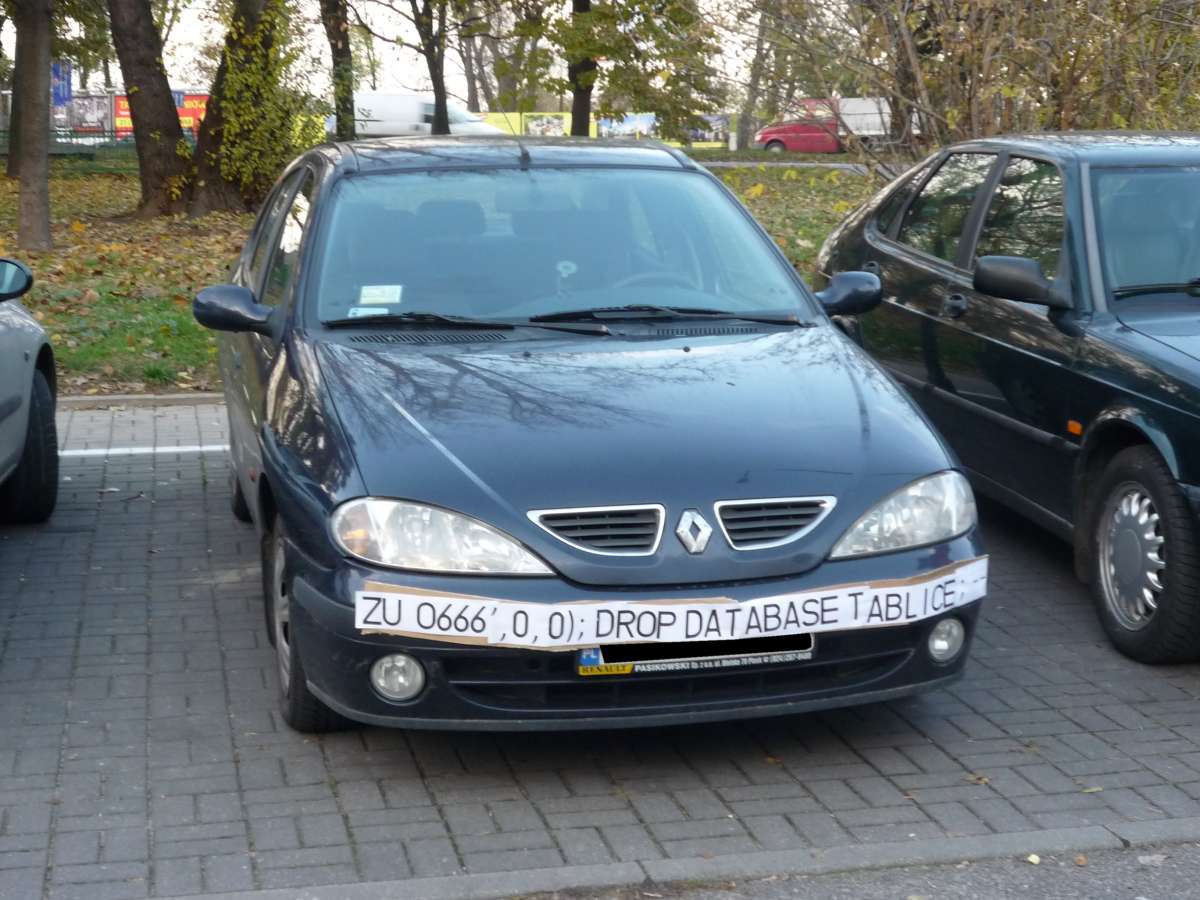
\includegraphics[width=\textwidth]{18mpenleoksq8jpg.jpg}
  \fontsize{10pt}{10pt}\selectfont
  \url{https://gizmodo.com/5498412/%
       sql-injection-license-plate-hopes-to-foil-euro-traffic-cameras}
\end{frame}


\begin{frame}{Autenticação quebrada}
  Já falamos bastante sobre senhas fracas e ataques de dicionário!
  \vfill
  Outros exemplos:
  \vfill
  \centering
  Recuperação de senha com KBA \\
  (\emph{Knowledge-Based Authentication}): \\
  perguntas sobre o usuário
  utilizando informações muitas vezes disponível publicamente
  (permite o ataque por terceiros)
  ou incorretas (\emph{bricking} para o próprio usuário).
  \vfill
  Hash fraco ou mal utilizado \\ (sem o ``sal'' / \emph{nonce}): \\
  \emph{Rainbow tables}, tabelas com valores pré-computados de hashes,
  podem ser utilizadas para reverter hashes,
  principalmente quando as mensagens são curtas
  (e.g. hashes de senhas).
\end{frame}


\begin{frame}[fragile]{Exemplo de falha de configuração no NGINX}
  \begin{minted}{nginx}
    upstream meu_servidor {
      server 127.0.0.1:5000 fail_timeout=0;
    }

    server {
      listen 80;
      location /static/ {
        alias /app/static_files/;
        expires 30d;
      }
      root /app;
      location / {
        try_files $uri @proxy_to_app;
      }
      location @proxy_to_app {
        proxy_set_header X-Forwarded-For $proxy_add_x_forwarded_for;
        proxy_set_header Host $http_host;
        proxy_redirect off;
        proxy_pass http://meu_servidor;
      }
    }
  \end{minted}
  Código do servidor em \texttt{/app} disponível para download?
  Inclusive arquivos como \texttt{.env} ou \texttt{settings.py}
  com credenciais?
\end{frame}


\begin{frame}[fragile]{Exposição de dados sensíveis}
  Banco de dados exposto?
  Solução tradicional:
  \emph{Firewall} bloqueando acesso à porta do banco
  + acesso via túnel SSH (\emph{Secure Shell})!
  \begin{minted}{shell}
    ssh -L 5432:db.server.com.br:5432 -v username@123.123.123.123
  \end{minted}
  \vfill\hrule\vspace{2pt}\hrule\vfill
  \centering
  Credenciais via HTTP ao invés de HTTPS?
  Qualquer um observando o tráfego da rede poderá ver sua senha!
  Há alternativas ``desesperadas''
  para tentar garantir a confidencialidade da senha
  mesmo sem HTTPS
  (e.g. roteador Linksys E2500
        troca a senha pelo hash no \emph{front-end}
        antes de enviar),
  mas, além de complicadas,
  não garantem a integridade do conteúdo e a identidade da fonte.
\end{frame}


\begin{frame}{Outros assuntos}
  \begin{itemize}
    \item Aspectos sociais/políticos (e.g. Manifesto Cypherpunk)
    \item Importância do FLOSS
          (\emph{Free/Libre Open Source Software}),
          padrões abertos e transparência
    \item TOR (\emph{The Onion Ring}),
          \url{https://www.torproject.org/}
    \item Detecção de [possíveis] fraudes (e.g. Serenata de Amor)
    \item \emph{Pentest} (\emph{penetration test}, teste de intrusão)
    \item \emph{Capture the flag}
    \item \emph{Firewall} e restrição de acesso
    \item DoS / DDoS (negação de serviço)
    \item DevSecOps
    \item ``Bugs famosos'' (Heartbleed, Meltdown, Spectre, ...)
  \end{itemize}
\end{frame}


\begin{frame}{Referências}
  \fontsize{9pt}{9pt}\selectfont
  A maioria do material está disponível apenas em inglês.
  \begin{itemize}
    \item Livro de GPG:
          \url{https://www.gnupg.org/gph/en/manual/book1.html}
    \item Tutorial de GPG:
          \url{https://www.futureboy.us/pgp.html}
    \item Página oficial do Tomb:
          \url{https://www.dyne.org/software/tomb/}
    \item Resumo sobre o Tomb:
          \url{https://pujol.io/blog/tomb-with-gpg-keys/}
    \item Página oficial do Pass:
          \url{https://www.passwordstore.org/}
    \item SHAttered:
          \url{https://shattered.io/}
    \item Repositório do gerador de certificados
          da Python Sudeste 2018:
          \url{https://github.com/danilobellini/certificados-pyse2018}
    \item Repositório da página da Python Sudeste 2018:
          \url{https://github.com/pythonsudeste/pythonsudeste2018-site}
    \item OWASP:
          \url{https://www.owasp.org/}
    \item OWASP 2017
          Top 10 most critical web application security risks:
          \url{https://github.com/OWASP/Top10/blob/master/2017/%
               OWASP\%20Top\%2010-2017\%20(en).pdf}
    \item RFC1991 (PGP, obsoleto):
          \url{https://tools.ietf.org/html/rfc1991}
    \item RFC4880 (OpenPGP):
          \url{https://tools.ietf.org/html/rfc4880}
    \item RFC4226 (HOTP):
          \url{https://tools.ietf.org/html/rfc4226}
    \item RFC6238 (TOTP):
          \url{https://tools.ietf.org/html/rfc6238}
  \end{itemize}
  \vfill\centering [... Continua no próximo slide ...]
\end{frame}


\begin{frame}{Referências}
  \fontsize{9pt}{9pt}\selectfont
  \begin{itemize}
    \item Trabalho ``Security vs safety'' do aluno
          Eirik Albrechtsen da NTNU, 2003:
          \url{http://www.iot.ntnu.no/users/albrecht/rapporter/%
               notat\%20safety\%20v\%20security.pdf}
    \item Time to rethink mandatory password changes:
          \url{https://www.ftc.gov/news-events/blogs/techftc/2016/03/%
               time-rethink-mandatory-password-changes}
    \item Want Safer Passwords? Don't Change Them So Often:
          \url{https://www.wired.com/2016/03/%
               want-safer-passwords-dont-change-often/}
    \item NIST is no longer recommending 2FA using SMS:
          \url{https://www.schneier.com/blog/archives/2016/08/%
               nist_is_no_long.html}
    \item Fixing the cell network flaw
          that lets hackers drain bank accounts
          \url{https://www.wired.com/2017/05/%
               fix-ss7-two-factor-authentication-bank-accounts/}
    \item Fixing the cell network flaw
          that lets hackers drain bank accounts
          \url{https://www.wired.com/2017/05/%
               fix-ss7-two-factor-authentication-bank-accounts/}
    \item Simple social engineering trick
          with a phone call and crying baby:
          \url{https://www.youtube.com/watch?v=lc7scxvKQOo}
    \item O que é desenvolvimento seguro, DevSecOps e S-SDLC
          (Communities Dev Show 2018):
          \url{https://www.slideshare.net/cassiobp/%
               o-que-desenvolvimento-seguro-devsecops-e-ssdlc}
  \end{itemize}
  Todas as imagens utilizadas nos slides sem fonte explícita
  foram obtidas do Wikipedia,
  exceto as do slide inicial,
  as quais foram obtidas em \url{http://etecuirapuru.com.br/}.
\end{frame}


\begin{frame}
  \begin{center}\fontsize{5cm}{2.5cm}\selectfont
    FIM!
  \end{center}
\end{frame}


\end{document}
